
\begin{figure}[H]
    \begin{center}
      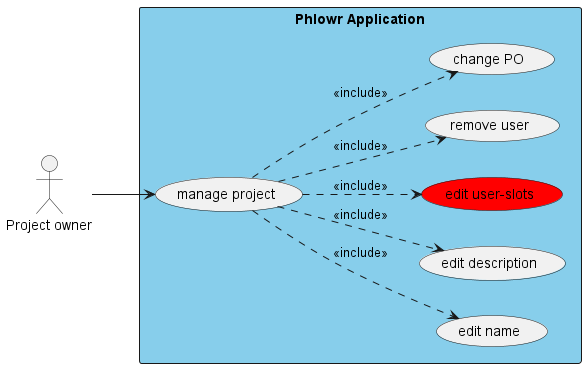
\includegraphics[width=0.3\linewidth]{../content/diagrams/usecase/manageProject/manageProjectUseCaseEditUserSlotsSelected.png}
      \caption{Use Case Diagaramm <edit user-slots> }
    \end{center}
  \end{figure}
  
\begin{table}[H]
    \centering
    \settowidth\tymin{executeIncomingCommand()}
    \setlength\extrarowheight{2pt}
    \begin{tabulary}{1.0\textwidth}{|m{4cm}|m{9cm}|}
      \hline
      \textbf{Use Case} &
      \textbf{EDIT USER-SLOTS}\\
      \hline
      \textbf{Beschreibung} &
      User-Slots des Projektes werden editiert\\ 
      \hline
      \textbf{Includes} &
      \begin{itemize}
       \item keine
        \end{itemize}\\  
      \hline
      \textbf{Akteure} &
      Projekt-Owner\\ 
      \hline
      \textbf{Auslöser} &
      \begin{itemize}
        \item ein Slot für einen neuen Entwickler wird benötigt
        \item ein Slot für einen neuen Entwickler wird nicht mehr benötigt
         \end{itemize}\\  
      \hline
      \textbf{Vorbedingungen} &
      \begin{itemize}
        \item Vorbedingungen vom <MANAGE PROJECT>-Use-Case
      \end{itemize}\\  
      \hline
      \textbf{Abschlussbedingunen} &
      Die Anzahl User-Slots wurde im Projekt angepasst und entsprechend gespeichert\\ 
      \hline
      \textbf{Ablauf} &
      \begin{enumerate}
        \item Applikation öffnen
        \item <Projekt Editieren> wählen
        \item + / - unter dem abschnitt <User-Slots> wählen
        \item Speichern
        \end{enumerate}\\ 
      \hline
      \textbf{Zu Beachten / Notizen} &
      \begin{itemize}
        \item keine
        \end{itemize}\\ 
      \hline
    \end{tabulary}
    \caption{Use Case: manage project -> EDIT USER-SLOTS}
  \end{table}